% Source for the figure of DirectAccessCodes (sec. 21.8): the sequence 5, 1,
% 18, 3, 260, 7, 40 in levels of chunks of 3 bits, each chunk with the bit
% that tells whether its integer continues, and the access to the item 4
% (shaded). Build: make figures (in ../build).
\documentclass[border=4pt]{standalone}
\usepackage[T1]{fontenc}
\usepackage{lmodern}
\usepackage{amsmath}
\usepackage{tikz}
\usepackage{lamalunga}
% tikz-ads.tex: the TikZ styles shared by the figures of the memory of the
% manual, \input by each standalone figure: a cell of a vector (cell), the
% cell that an operation touches (touched), a free cell (free), a node of a
% linked structure (node), the labels of indices (index) and of variables
% (var), a pointer (ptr), and \cells and \indices to draw a row of cells.
\usetikzlibrary{arrows.meta,positioning,calc,fit,shapes.multipart}
\definecolor{adsTouched}{RGB}{214,196,236}
\definecolor{adsFree}{RGB}{236,236,236}
\tikzset{
  ads/.style={>={Stealth[length=2mm]},font=\small,
              every node/.append style={inner sep=0pt}},
  cell/.style={draw,minimum width=7mm,minimum height=7mm,
               font=\small\ttfamily,outer sep=0pt},
  touched/.style={cell,fill=adsTouched},
  free/.style={cell,fill=adsFree,text=black!45},
  node/.style={draw,rounded corners=1pt,minimum width=8mm,
               minimum height=6mm,font=\small\ttfamily},
  index/.style={font=\scriptsize\ttfamily,text=black!60},
  var/.style={font=\small\itshape},
  ptr/.style={->,thick}
}
% \cells{name}{x,y}{list}: a row of cells, the first at (x,y), named
% name-0, name-1, ...; each item is text/style, the style one of cell,
% touched and free (e.g., {a/cell,e/touched,/free})
\newcommand{\cells}[3]{%
  \foreach \v/\s [count=\i from 0] in {#3}
    \node[\s] (#1-\i) at ($(#2)+(\i*7mm,0)$) {\v};}
% \indices{name}{n}: the indices 0 .. n-1 under the cells of name
\newcommand{\indices}[2]{%
  \foreach \i in {0,...,\numexpr#2-1\relax}
    \node[index,below=1.2mm of #1-\i] {\i};}

\begin{document}
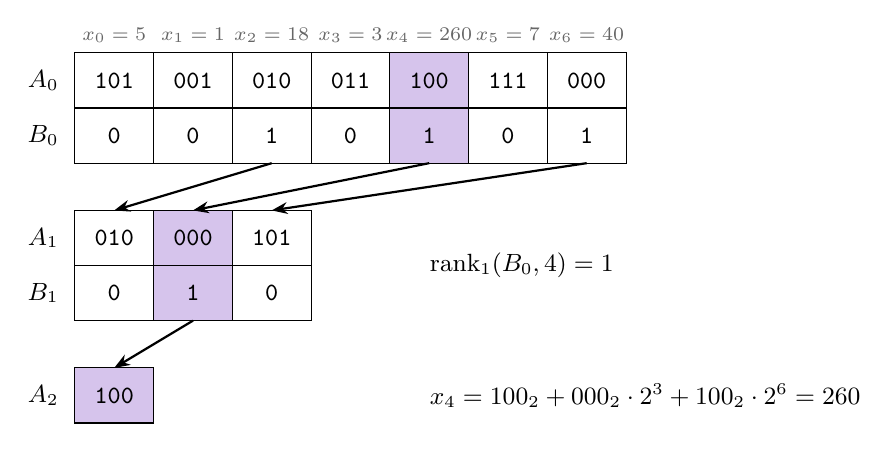
\begin{tikzpicture}[ads,c/.style={cell,minimum width=10mm},
                       t/.style={touched,minimum width=10mm}]
  % level 0: the low chunk of every integer
  \node[var,anchor=east] at (-7mm,0) {$A_0$};
  \node[var,anchor=east] at (-7mm,-7mm) {$B_0$};
  \foreach \v/\s [count=\i from 0] in {101/c,001/c,010/c,011/c,100/t,111/c,000/c}
    \node[\s] (a0-\i) at (\i*10mm,0) {\v};
  \foreach \v/\s [count=\i from 0] in {0/c,0/c,1/c,0/c,1/t,0/c,1/c}
    \node[\s] (b0-\i) at (\i*10mm,-7mm) {\v};
  \foreach \x [count=\i from 0] in {5,1,18,3,260,7,40}
    \node[index,above=1.2mm of a0-\i] {$x_{\i} = \x$};
  % level 1: the integers of more than 3 bits
  \node[var,anchor=east] at (-7mm,-20mm) {$A_1$};
  \node[var,anchor=east] at (-7mm,-27mm) {$B_1$};
  \foreach \v/\s [count=\i from 0] in {010/c,000/t,101/c}
    \node[\s] (a1-\i) at (\i*10mm,-20mm) {\v};
  \foreach \v/\s [count=\i from 0] in {0/c,1/t,0/c}
    \node[\s] (b1-\i) at (\i*10mm,-27mm) {\v};
  % level 2: the integers of more than 6 bits
  \node[var,anchor=east] at (-7mm,-40mm) {$A_2$};
  \node[t] (a2-0) at (0,-40mm) {100};
  % the integers that continue, and the place of each at the next level
  \foreach \f/\t in {2/0,4/1,6/2}
    \draw[ptr] (b0-\f.south) -- (a1-\t.north);
  \draw[ptr] (b1-1.south) -- (a2-0.north);
  \node[var,anchor=west] at (40mm,-23.5mm)
    {$\mathrm{rank}_1( B_0 , 4 ) = 1$};
  \node[var,anchor=west] at (40mm,-40mm)
    {$x_4 = 100_2 + 000_2 \cdot 2^3 + 100_2 \cdot 2^6 = 260$};
\end{tikzpicture}
\end{document}
